\documentclass[]{elsarticle} %review=doublespace preprint=single 5p=2 column
%%% Begin My package additions %%%%%%%%%%%%%%%%%%%
\usepackage[hyphens]{url}

  \journal{Global Change Biology (?)} % Sets Journal name


\usepackage{lineno} % add
\providecommand{\tightlist}{%
  \setlength{\itemsep}{0pt}\setlength{\parskip}{0pt}}

\bibliographystyle{elsarticle-harv}
\biboptions{sort&compress} % For natbib
\usepackage{graphicx}
\usepackage{booktabs} % book-quality tables
%%%%%%%%%%%%%%%% end my additions to header

\usepackage[T1]{fontenc}
\usepackage{lmodern}
\usepackage{amssymb,amsmath}
\usepackage{ifxetex,ifluatex}
\usepackage{fixltx2e} % provides \textsubscript
% use upquote if available, for straight quotes in verbatim environments
\IfFileExists{upquote.sty}{\usepackage{upquote}}{}
\ifnum 0\ifxetex 1\fi\ifluatex 1\fi=0 % if pdftex
  \usepackage[utf8]{inputenc}
\else % if luatex or xelatex
  \usepackage{fontspec}
  \ifxetex
    \usepackage{xltxtra,xunicode}
  \fi
  \defaultfontfeatures{Mapping=tex-text,Scale=MatchLowercase}
  \newcommand{\euro}{€}
\fi
% use microtype if available
\IfFileExists{microtype.sty}{\usepackage{microtype}}{}
\usepackage{graphicx}
% We will generate all images so they have a width \maxwidth. This means
% that they will get their normal width if they fit onto the page, but
% are scaled down if they would overflow the margins.
\makeatletter
\def\maxwidth{\ifdim\Gin@nat@width>\linewidth\linewidth
\else\Gin@nat@width\fi}
\makeatother
\let\Oldincludegraphics\includegraphics
\renewcommand{\includegraphics}[1]{\Oldincludegraphics[width=\maxwidth]{#1}}
\ifxetex
  \usepackage[setpagesize=false, % page size defined by xetex
              unicode=false, % unicode breaks when used with xetex
              xetex]{hyperref}
\else
  \usepackage[unicode=true]{hyperref}
\fi
\hypersetup{breaklinks=true,
            bookmarks=true,
            pdfauthor={},
            pdftitle={Functional resistance to a selective logging disturbance in Amazonian forests},
            colorlinks=false,
            urlcolor=blue,
            linkcolor=magenta,
            pdfborder={0 0 0}}
\urlstyle{same}  % don't use monospace font for urls

\setcounter{secnumdepth}{0}
% Pandoc toggle for numbering sections (defaults to be off)
\setcounter{secnumdepth}{0}
% Pandoc header



\begin{document}
\begin{frontmatter}

  \title{Functional resistance to a selective logging disturbance in Amazonian
forests}
    \author[1]{Camille Piponiot\corref{c1}}
   \ead{camille.piponiot@gmail.com} 
   \cortext[c1]{Corresponding Author}
    \author[]{TmFO authors}
  
  
    \author[1, 2]{Bruno Hérault}
   \ead{bruno.herault@cirad.fr} 
  
      \address[1]{Cirad, UR Forets et Societes, Montferrier-sur-Lez, France}
    \address[2]{INPHB, Yamoussoukro, Cote d'Ivoire}
  
  \begin{abstract}
  Tropical forests bring numerous benefits for humanity, but they suffer
  from increasing human disturbance that can lastingly modify their
  functioning. In this study we evaluate the effect of selective logging,
  one of the most widespread human disturbances in tropical forests, on
  Amazonian forests' functional composition. We develop a model of
  post-logging trajectory of community weighted mean traits and calibrate
  it in a Bayesian framework using data from 12 experimentally logged
  sites (264 ha total) spread over the Amazon biome. We test the effect of
  the initial composotion and functional diversity as well as the
  precipitation seasonality and stem turnover rate on the functional
  resistance to a logging disturbance (i.e.~the maximum relative change in
  functional composition after logging).
  
  Our results show that, contrary to expectations, the intital composition
  and functional diversity have no significant effect on the functional
  resistance in our plots. The stem turnover rate was the best predictor
  of post-logging resistance for two traits, namely the
  95\textsuperscript{th} percentile of a species diameter distribution (as
  a proxy of adult tree stature) and wood density. Forests with high
  turnover rates were predicted to be the more resistant to logging.
  Overall, adult tree stature and SLA seem to be more resistant to
  logging, while seed mass and wood density show consistent decreases
  after a logging disturbance. Forests in northeastern Amazonia are
  predicted to experience the strongest decreases in wood density after
  logging (-10\%). These forests are especially important for water cycles
  and carbon sequestration, and a decrease in wood density may lower their
  ability to provide these benefits.
  \end{abstract}
  
 \end{frontmatter}

\section{Introduction}\label{introduction}

Tropical forests are crucial for most global ecological cycles. They
hold 230 Pg of carbon, around 11\% of the total carbon in terrestrial
ecosystems (Baccini et al. 2012) and intact tropical forests are
estimated to have sequestered an annual 1.19 \(\pm\) 0.41 Pg of carbon
between 1990-2007 (Pan et al. 2011), about 15\% of total anthropogenic
carbon emissions, thus playing a major role in climate change mitigation
(IPCC 2014). Tropical forests are also key in the global water cycle,
recycling rainfall through vegetation evapotranspiration and thus
buffering droughts in adjacent regions (Staal et al. 2018). Moreover,
tropical forests harbor an exceptional biodiversity (Jenkins, Pimm, and
Joppa 2013,Slik et al. (2015)), providing species to surrounding regions
through biotic interchanges (Antonelli et al. 2018). The state of
tropical forests thus largely determines the functioning of global
ecosystems, and hence human well-being.

The future of tropical forests is however highly uncertain: during the
past three centuries, humans activities have triggered rapid changes in
global ecosystems, causing massive species extinctions and accelerating
climate change through increased carbon emissions (Crutzen 2002). During
the past century these changes are particularly intense in the tropics,
where forests are being clearcut for agricultural or mining purposes at
unprecedented rates, and where most remaining forests have or will be
heavily impacted by human activities (Malhi et al. 2014).

One predominant human activity in tropical forests is the selective
logging of a few merchantable trees: around 400 million hectares of
tropical forests are designated for timber production (Blaser et al.
2011), and ca. 20\% of tropical forests were affected by selective
logging between 2000 and 2005 (Asner et al. 2009). Because selective
logging focuses on a few individual trees (typically 5-10 trees per
hectare), 65-95\% of the forest cover is maintained after logging
operations (Cannon et al. 1994,Pereira et al. (2002)). Damage to the
forest is concentrated in logging gaps created by tree felling, and in
infrastructure (skid trails and, to a lesser extent, roads and log
decks) (Pereira et al. 2002,Asner, Keller, and Silva (2004)).

Disturbances such as selective logging, droughts, fires, or hunting, are
increasing in intensity and frequency (Lewis, Edwards, and Galbraith
2015). Human disturbances alter the composition and dynamics of tropical
forests by provoking a higher-than-normal tree mortality, which can
affect some trees more than others. Large trees of commercial value with
good mechanical properties are the focus of loggers; trees with
low-density wood are more vulnerable to droughts (Mcdowell et al.
2018,Aleixo et al. (2019)), and trees with thick bark are more resistant
to fires (Brando et al. 2012). Directional mortality has a
strait-forward effect on forest composition and structure. The indirect
effect of disturbance is the higher recruitment of light-demanding
species in canopy gaps (Carreño-Rocabado et al. 2012): these changes in
tree species composition can last for several decades (Avila et al.
2015).

Changes in composition and their effects on forest functioning can be
quantified with functional traits (Chapin III et al. 1997,Lavorel and
Garnier (2002)). Functional traits are measures of an individual's
features that impact its growth, reproduction and survival, and hence
its overall fitness (Violle et al. 2007). In tropical forests, at least
four major functional axes have been described: (i) the leaf economic
spectrum (short-lived low-investment leaves vs.~tough leaves) (Wright et
al. 2004), the wood economic spectrum (fast-growing low-density
vs.~long-lived high-density wood) (Chave et al. 2009), adult tree
stature and height (canopy vs.~understory trees) linked to light capture
(Poorter et al. 2003) and survival strategy (Johnson et al. 2018), and
the seed dispersal strategy (large, zoochorous and resource-rich seeds
vs.~light anemochorous seeds) (Poorter and Rose 2005). Together, these
four axes explain most of the functional variation observed in forest
ecosystems (Baraloto, Hardy, et al. 2012,Costa-Saura et al. (2019)).

Disturbances such as selective logging change local conditions by
creating canopy gaps and thus increasing the quantity of light that gets
to the soil. The new light conditions favor the germination and rapid
growth of small-seeded, light-wooded species (Poorter and Rose
2005,Baraloto, Hérault, et al. (2012),Baker et al. (2016),Poorter et al.
(2019)). These light-demanding pioneer species have high growth rates
but generally poor resistance to drought (Aleixo et al. 2019). It has
also been shown that selective logging can decrease the canopy height,
and consequently total carbon storage (Rutishauser et al. 2016).
Understanding the long-term effects of disturbances on a community's
functional composition will thus be key to predict the future of
tropical forests in the context of rapid changes in disturbance regimes
(Wright 2005).

Ecosystem resilience is a measure of an ecosystem's ability to cope with
disturbances (Holling 1973). It is a key concept to understand the
long-term changes in forest composition and dynamics following a
disturbance. The notion of resilience can be defined with two essential
components: the change in state (or resistance to disturbance), and the
time to return to a pre-disturbance state (or recovery) (Hodgson,
McDonald, and Hosken 2015). Resilience, and in particular its
change-in-state component, depends strongly on the disturbance frequency
and intensity. Additionally, ecological memory of past disturbances is a
key component of forest resilience (Johnstone et al. 2016,Ciemer et al.
(2019)). Ecological memory translates into the presence and diversity of
trees and seeds of species with life-history traits adapted to
disturbances, which in turn can shape forest demographics, and
especially vegetation turnover rates (Lavorel and Garnier
2002,({\textbf{???}})). Environmental constraints such as water
limitations have also been shown to affect the functional resistance of
Neotropical forests to disturbances ({\textbf{???}}).

In Amazonia, the largest tropical forest biome on Earth (600 million
hectares), at least two large gradients explain regional patterns of
forest dynamics (Johnson et al. 2016). Vegetation productivity is
strongly correlated to the precipitation regime (Fauset et al. 2019),
being higher in northwestern forests with high levels of precipitation
and lower in southeastern forests which suffer from a long dry season
(Davidson et al. 2012,Johnson et al. (2016)). Stem turnover rates
describe a Northeast-Southwest gradient ({\textbf{???}}), mainly driven
by soil stability (Quesada et al. 2012), and the frequency and intensity
of natural disturbances such as windstorms (Espírito-Santo et al.
2014,Negrón-Juárez et al. (2018)) and droughts (Phillips et al. 2010).
Understanding how these gradients structure the forest response to a
logging disturbance can help improve predictions of Amazonian forests
vulnerability to future increases in disturbance regimes.

Here we assess the resistance of four functional traits (namely wood
density, seed mass, specific leaf area and maximum tree diameter) to
selective logging in Amazonia. Our research questions are: (i) how is
the functional composition of Amazonian forests affected by disturbances
such as selective logging? (ii) are some functional traits more
resistant than others? (ii) what is the effect of initial functional
composition and diversity on the functional resistance? and (iv) how
does functional resistance vary across Amazonia, and is it related to
regional patterns of natural disturbances?

To bring light on these questions, we modeled the post-disturbance
trajectory of four key community mean traits within an original Bayesian
hierarchical model. We calibrated the model using data from 161
permanent forest plots from 12 long-term experimentally logged sites
(264 ha total) spread over Amazonia. We tested the effect of the initial
(pre-disturbance) trait value and functional diversity, and of regional
patterns of forest demographics (stem turnover rate as a proxy of
natural disturbance regimes) and precipitation seasonality.

\section{Methods}\label{methods}

\subsection{Study sites}\label{study-sites}

\begin{figure}
\centering
\includegraphics{rticle_tmfo_functional_files/figure-latex/map_tmfo_sites-1.pdf}
\caption{\label{fig:map_tmfo}Location of the 12 experimental permanent
forest sites used in this study: the size of the points represents the
total monitored area, and the color (from yellow to red) represents the
total length of the experiment, as the time interval (in years) between
the first and the last census. Grey boundaries define 6 ecoregions and
were retrieved from Ter Steege et al., 2013 (Ter Steege et al. 2013),
CA: central Amazonia, EA: eastern Amazonia, GS: Guiana shield, SEA:
southeastern Amazonian, SWA: southewestern Amazonia, and WA: western
Amazonia. Green areas define the Amazonian biome.}
\end{figure}

Our study includes data from twelve long-term (8--35 year) experimental
forest sites located in the Amazon Basin and the Guiana Shield (Figure
\ref{fig:map_tmfo}) (Sist et al. 2015). All sites are located in
tropical forests with mean annual precipitation \(\geq\) 1000 mm. In
each site, permanent forest plots (3-56.25 ha per site) were logged, and
censused at least once before and twice after logging.

For each site, we extracted the precipitation seasonality from Worldclim
database (bioclimatic variable 15) (Fick and Hijmans 2017), at a 2.5
arc-minute resolution. Annual stem turnover rates (as a \% of live
stems) were based on data from unlogged plots inside our sites. For the
5 sites in which no unlogged plot was available, stem turnover rates
were extracted from a map based on the metadata from Johnson and
colleagues (Johnson et al. 2016) (extracted from the ForestPlots
database (Lopez-Gonzalez et al. 2011)) and interpolated with the R
package gstat (Pebesma 2004) on a 1\(^\circ\) resolution grid. Site
coordinates, precipitation seasonality and stem turnover rates are
reported in Table \ref{tab:sites}.

\subsection{Data compilation}\label{data-compilation}

For sites with plots \(\leq\) 1 ha, data from those with the same
treatment were aggregated to mitigate the small plot effect on the
variation in density of large trees. In each census, all trees \(\geq\)
10 cm diameter at breast height (dbh) were marked, measured and
identified to the lowest taxonomic level (84\% to species, 14\% to
genus).

Median values of functional traits were calculated at the species level.
Four functional traits were chosen, as proxies of complementary
ecosystem functions in tropical forests: (i) the DBH 95th percentile as
a proxy of adult tree stature and light demand (Poorter et al. 2003),
(ii) the seed mass (log-transformed) as a proxy of the dispersal
strategy (Poorter and Rose 2005), (iii) the specific leaf area as a
proxy of the assimilation strategy and leaf economic spectrum (Wright et
al. 2004) and (iv) the stem wood density as a proxy of growth rate and
mechanical support (Chave et al. 2009).

The DBH 95th percentile was chosen because it is more robust than the
maximum DBH which is too sensitive to sampling size. The DBH 95th
percentile was calculated for all species for which at least 20
individuals were censused in our permanent forest plots. Seed mass and
specific leaf area measurements were retrieved from the TRY database
(Kattge et al. 2011) (datasets citations xx). Wood density measurements
were retrieved from the global wood density database (Chave et al.
2009,Zanne et al. (2009)).

Median trait values were calculated per species and genus. Each
individual tree in our permanent sample plots was then attributed a
value for each trait at the lowest available taxonomic level. Trees with
no available species- or genus-specific trait value were given their
plot's median trait value. The aboveground biomass of each individual
was estimated using the R package BIOMASS (Réjou-Méchain et al., n.d.).

Selective logging typically targets large trees belonging to a small
group of species with commercial value. Those species usually have
particular functional trait values, such as large maximum diameters. The
functional composition of the largest trees is thus artificially
modified because of the selectivity of harvests. Because we are more
interested in the indirect effects of selective logging disturbance on
the functional composition, i.e.~the functional changes induced by tree
felling and canopy openings, we excluded large trees with DBH
\textgreater{} 35 cm from the analysis.

For each functional trait \(k\) (either \(DBH95\), \(logSeedMass\),
\(SLA\), or \(WD\)), we computed the community's mean biomass-weighted
trait (CMT) value at census \(c\) in plot \(p\) in site \(s\) as:

\begin{equation}  
CMT_{k,c,p,s} = \frac{\sum_{i \in I_{c,p,s}}(T_{k,i}\cdot agb_i)}{\sum_{i \in I_{c,p,s}}(agb_i)}
\end{equation}

with \(T_{k,i}\) the value of trait \(k\) for individual tree \(i\),
\(agb_i\) the aboveground biomass of individual tree \(i\), and
\(I_{c,p,s}\) all live trees with DBH \(\geq\) 10 cm and \(\leq\) 35 cm
at census \(c\) in plot \(p\) in site \(s\). Mean trait values were
weighted by aboveground biomass to reflect the importance of larger
trees in forest functioning (e.g.~carbon cycling).

The distance of a trait value to its initial (pre-logging) value was
estimated as:

\begin{equation}  
dCMT_{k,c,p,s} = \frac{CMT_{k,c,p,s} - CMT0_{k,p,s}}{CMT0_{k,p,s}}
\end{equation}

The functional diversity \(FD_{k,c,p,s}\) for a given trait \(k\) was
calculated as the similarity-based diversity of order 1 of all trees
with dbh between 10 and 35 cm at census \(c\) in plot \(p\) and site
\(s\), and was calculated with the function \(Dqz\) in the R package
\emph{entropart} (Marcon and Hérault 2015).

\subsection{Model calibration}\label{model-calibration}

The model presented here aims at capturing the changes in the
community's mean biomass-weighted traits (CMT) after the disturbance, as
well as their recovery. For each trait \(k\), the change in CMT at
census \(c\) in plot \(p\) and site \(s\) was modeled as:

\begin{equation}  
dCMT_{k,c,p,s} \sim \mathcal{N}\left( \mu_{k,c,p,s}\text{ , } \left(\frac{\sigma_k}{size_p}\right)^2\right)
\end{equation}

where

\begin{equation}  
\mu_{k,c,p,s} = \Delta_{k,p,s} \cdot \left( \frac{t_c}{tmax_{k,p,s}} \cdot exp\left(1-\frac{t_c}{tmax_{k,p,s}}\right) \right)^{\theta_{k,p,s}}
\end{equation}

with \(t_c\) the time since logging (in years) at census \(c\);
\(size_p\) is the size of plot \(p\); \(\Delta_{k,p,s}\) is the maximum
post-disturbance change (negative if the CMT decreases, and positive of
it increases). \(tmax_{k,p,s}\) is the time taken to reach
\(\Delta_{k,p,s}\); when \(t_c > tmax_{k,p,s}\), the CMT starts to get
closer to its initial value, entering the recovery phase which is in
some plots not yet observed. \(\theta_k\) is a shape parameter that
controls the width of the hump; when it increases, the hump is narrower.

Parameters \(\Delta_{k,s,p}\) and \(tmax_{k,p}\) were modeled with a
normal distribution:

\begin{equation}
tmax_{k,p,s} \sim \mathcal{N} (\mu m1_{s,k}, \sigma m1^2)
\end{equation}

where \(\sigma m1\) is the standard deviation of \(tmax\) and
\(\mu m1_{s,k}\) is the mean of \(tmax\) for trait \(k\) in site \(s\).
To benefit from the information from sites with long experiment duration
and help infer \(tmax\) in sites where it had not been reached during
the experiment duration (i.e.~no observed return to initial CMT because
of short experiment duration), we added one hierarchical level to
\(tmax\):

\begin{equation}
\mu m1_{s,k} \sim \mathcal{N} (\mu m2_{k}, \sigma m2^2)
\end{equation}

with \(\mu m2_{k}\) and \(\sigma m2\) the mean and standard deviation of
\(\mu m1{s,k}\).

\begin{figure}
\centering
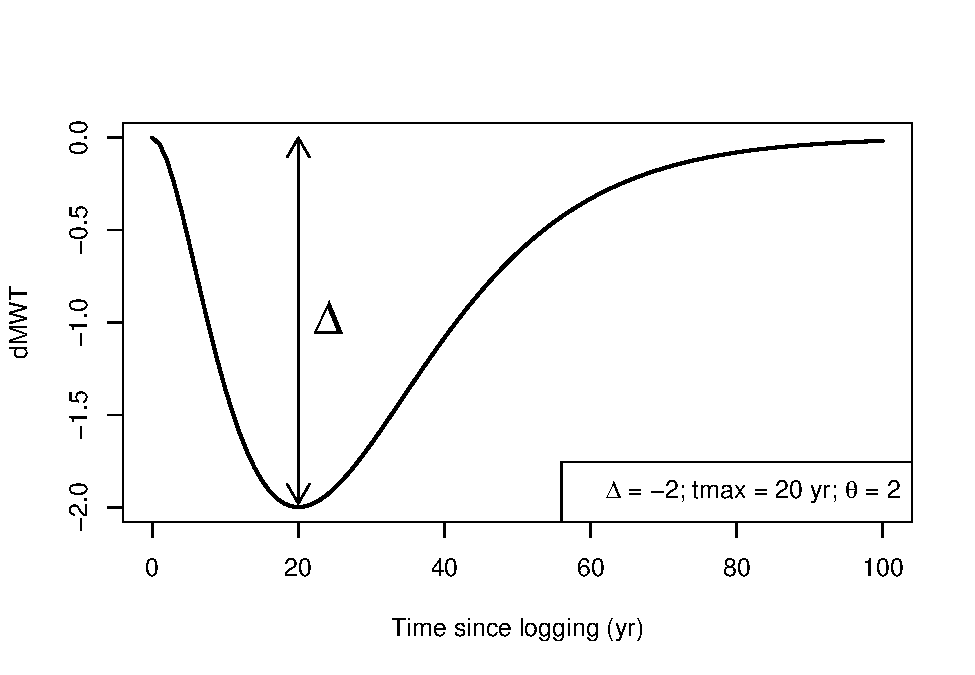
\includegraphics{rticle_tmfo_functional_files/figure-latex/method_example-1.pdf}
\caption{Example of predicted relative CMT change (dCMT) after a
disturbance.}
\end{figure}

\(\Delta_{k,p,s}\) is the maximum change of trait \(k\) after the
disturbance: its absolute value is expected to increase with disturbance
intensity. We thus modeled it as:

\begin{equation} 
\Delta_{k,p,s} \sim \mathcal{N} \left( loss_p \cdot (\lambda_{0,k} + \sum \lambda_{m,k} Cov_{m,k,p,s} )  , \sigma_{\Delta}^2 \right)
\end{equation}

where \(loss_p\) is the relative aboveground biomass loss after logging
in plot \(p\), as a proxy of the disturbance intensity; it is estimated
as the difference between the pre-logging aboveground biomass and the
minimum biomass in the first 4 years after logging, divided by the
pre-logging aboveground biomass (similar to Piponiot et al. (2016)).
\(Cov_{m,k,p,s}\) is the value of covariate \(m\) for trait \(k\) in
plot \(p\) in site \(s\). Covariates are (i) the stem turnover rate,
(ii) the precipitation seasonality (both defined for each site from
Amazonian-wide maps), (iii) the initial community mean trait and (iv)
the initial functional diversity, both defined for each trait and plot
with pre-logging censuses. \(\sigma_{\Delta}\) is the standard deviation
of \(\Delta\) for trait \(k\) in site \(s\).

Bayesian hierarchical models were inferred through MCMC methods using an
adaptive form of the Hamiltonian Monte Carlo sampling using the R
language (R Developement Core Team 2018) and the Rstan package
(Carpenter et al. 2017). A detailed list of priors is provided in Table
XXX (informative priors?).

\subsection{Predictions}\label{predictions}

Predictions of maximum CMT change after the disturbance were made at the
Amazonian level on a 1\(^\circ\) grid, i.e.~the coarsest resolution of
input maps, and errors were propagated with the following steps:

\begin{enumerate}
\def\labelenumi{\arabic{enumi}.}
\item
  For each cell \(j\) of the grid: (i) a value of stem turnover was
  taken from the map of stem turnover fitted with the data from (Johnson
  et al. 2016) (see (Piponiot et al. 2019)); (ii) a value of
  precipitation seasonality was taken from the distribution of pixel
  values in the Worldclim map (Fick and Hijmans 2017) that were inside
  the cell.
\item
  Parameters \(\lambda_{0,k}\) and \(\lambda_{m,k}\) were taken from
  their posterior distribution.
\item
  For each trait \(k\) and grid cell \(j\), predictions of maximum CMT
  change \(\Delta_{k,j}\) after a disturbance were calculated using a
  biomass loss of \(loss =\) 40\%:

  \begin{equation} 
  \label{eq:lambdas}
  \Delta_{k,j} = loss \cdot (\lambda_{0,k} + \sum \lambda_{m,k} Cov_{m,j}) 
  \end{equation}
\end{enumerate}

These steps were repeated 1000 times and summary statistics were
calculated for each 1\(^\circ\) grid cell.

\section{Results}\label{results}

\subsection{Predictions of functional trajectories and
parameters}\label{predictions-of-functional-trajectories-and-parameters}

\begin{figure}
\centering
\includegraphics{rticle_tmfo_functional_files/figure-latex/fig_tmax-1.pdf}
\caption{\label{fig:tmax_delta}Posterior distribution of parameters
\emph{tmax} (left panels) and Delta (right panels) per site (x-axis) and
trait (top to bottom panels). The wider the posterior, the larger the
uncertainty on its estimation. Functional traits are: \emph{DBH95}
community mean 95th percentile of the diameter at breast height (a proxy
of the adult stature); \emph{logSeedMass} community mean seed mass
(log-transformed); \emph{SLA} community mean specific leaf area;
\emph{woodDensity} community mean wood density. Ecoregions (as defined
in Ter Steege et al., 2013) are: CA: central Amazonia, EA: eastern
Amazonia, GS: Guiana shield, SWA: southewestern Amazonia and WA: western
Amazonia.}
\end{figure}

The estimated time to reach the maximum trait change is similar between
traits (Figure \ref{fig:tmax_delta}) and is estimated to be between
{[}5, 36{]} yr (95\% confidence interval).

The maximum relative trait change (\(\Delta\)) was between {[}-11,
7{]}\%, with large differences between traits and sites (Figure
\ref{fig:tmax_delta}). The community mean adult tree stature
(\emph{DBH95}) decreased after the disturbance in almost all sites
except the two sites in Bolivia: La Chonta and, to a lesser extent, INPA
(Figure \ref{fig:tmax_delta}). The community mean seed mass
(\emph{logSeedMass}) decreased in most sites after the disturbance
(\(\Delta \in\) {[}-19, 3{]}\%), except for two sites in western
Amazonia, Cumaru and Chico Bocão. The community mean specific leaf area
(\emph{SLA}) increased or stayed close to its initial value in most
sites after the disturbance, except in INPA, Bolivia (see full
trajectories in supplementary Figure \ref{sfig:pred_traj}). The increase
in the community mean SLA was especially high in Tapajos where it gained
+12\% compared to its initial value. The community mean wood density
(\emph{woodDensity}) decreased in most sites after the disturbance
(\(\Delta \in\) {[}-12, 1{]}\%), except for three sites: INPA, Peteco
and Tabocal, where it stayed close to its initial value.

\subsection{Effect of covariates on functional
resistance}\label{effect-of-covariates-on-functional-resistance}

\begin{figure}
\centering
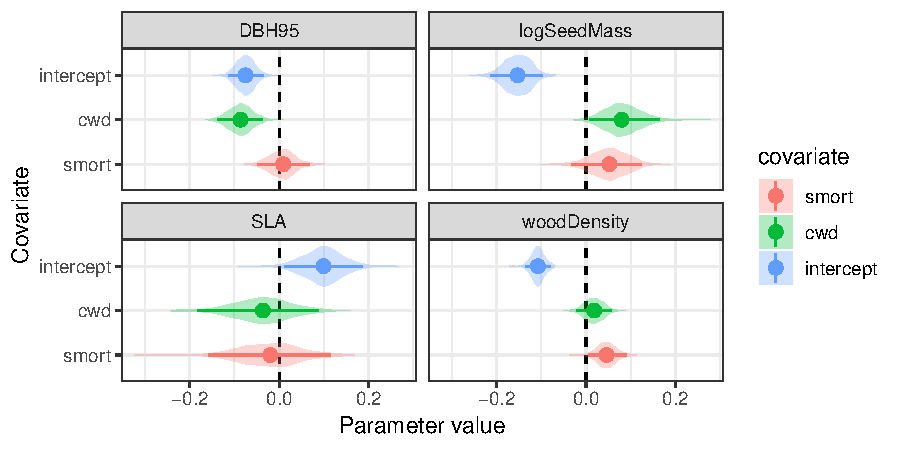
\includegraphics{rticle_tmfo_functional_files/figure-latex/lambdas-1.pdf}
\caption{\label{fig:lambdas}Covariates effect on maximum relative CMT
change per trait. \emph{intercept} is the value when all covariates are
null; \emph{seasonality} is the effect of the precipitation seasonality;
\emph{turnover} is the effect of the stem turnover rate; \emph{CMT} is
the effect of the initial community wbiomass-weighted mean trait; and
\emph{FD} is the effect of the initial functional diversity. Dots
represent the median value, and the segments are the 95\% confidence
intervals. All covariates were scaled and centered. Colours indicate if
zero is in the confidence interal: black when zero is in the 80\%
interval, dark blue when its in the 958\% interval but not the 80\%
interval, and light blue when its in neither.}
\end{figure}

The intercept \(\lambda0\) is significantly different from zero for all
traits except for \emph{DBH95} (Figure \ref{fig:lambdas}). A site with
average stem turnover rate and precipitation seasonality is thus
predicted to have a small non-significant decrease in \emph{DBH95} (as a
proxy of tree stature). Both the seasonality of precipitations and the
stem turnover rate have a significant positive effect on mean
\emph{DBH95}: highly seasonal forests with high turnover rates are
predicted to favor larger trees (on average) after a logging
disturbance, while forests with low precipitation seasonality and
turnover rates are predicted to have a decrease in mean \emph{DBH95}.
The initial functional composition (\emph{CMT}) and diversity
(\emph{FD}) have no significant effect on post-disturbance \emph{DBH95}
changes. The intercept is significantly negative for \emph{logSeedMass}
and positive for \emph{SLA}, but no significant covariate effect was
detected for either of these traits (Figure \ref{fig:lambdas}): seed
mass is predicted to decrease and SLA is predicted to increase after a
logging disturbance. For \emph{woodDensity}, the intercept is
significantly negative: wood density is predicted to decrease after a
logging disturbance (Figure \ref{fig:lambdas}). The effect of
precipitation seasonality is significantly negative and the effect of
stem turnover rate and the initial wood density (\emph{CMT}) have a
significantly positive effect on post-disturbance wood density change. A
forest with high precipitation seasonality, low stem mortality and low
initial wood density is thus predicted to have a stronger decrease of
mean wood density after a logging disturbance.

\subsection{Predictions of regional variability in functional
resistance}\label{predictions-of-regional-variability-in-functional-resistance}

\begin{figure}
\centering
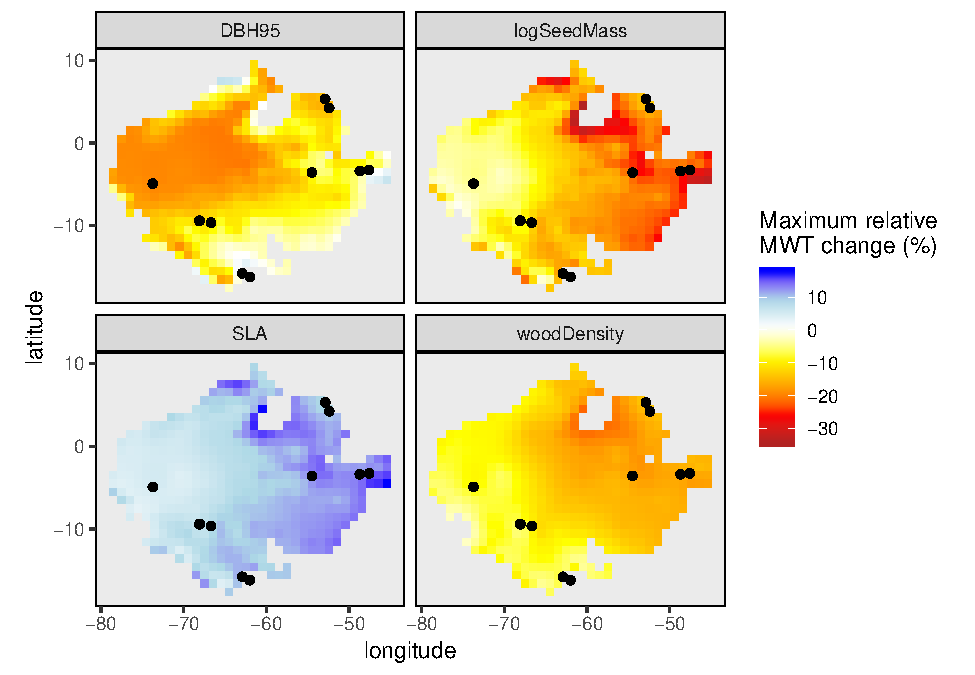
\includegraphics{rticle_tmfo_functional_files/figure-latex/maps_pred-1.pdf}
\caption{\label{fig:predmap}Prediction maps of maximum relative
community mean trait (CMT) change (i.e.~resistance to disturbance) by
trait. Warm colors (from yellow to red) show a decreases in CMT; blue
colors show an increase in CMT. Black dots are study sites location.}
\end{figure}

Functional resistance is predicted to vary strongly between traits and
across the Amazonian biome (Figure \ref{fig:predmap}). \emph{DBH95} is
predicted to decrease strongly in northern regions of Amazonia (up to
-\texttt{r}xx), and to increase slightly in the most southern regions of
Amazonia (Figure \ref{fig:predmap}a). Seed mass is predicted to strongly
decrease everywhere in Amazonia after selective logging, and especially
in southeastern regions (Figure \ref{fig:predmap}b). SLA is predicted to
increase, and in particular in southern Amazonia, except in northern
regions where it is expected to decrease slightly (Figure
\ref{fig:predmap}c). Wood density is predicted to decrease everywhere in
Amazonia after logging, ans especially in northeastern and eastern
Amazonia (Figure \ref{fig:predmap}d).

\section{Discussion}\label{discussion}

\subsection{Model structure and
limitations}\label{model-structure-and-limitations}

This study presents, to our knowledge, the first explicit model of
post-disturbance stand-level functional trajectory in tropical forests.
This model describes two phases of the trajectory: first a change in the
functional composition (\(t_c \in [0,tmax]\)) triggered by an increase
light availability that favors fast-growing pioneer trees, and second a
progressive return to initial functional composition (\(t_c > tmax\))
once the canopy gaps have closed and pioneer trees start to die. The
advantage of this framework is that it relies on a small set of
parameters to describe the trajectory, while accurately predicting
observations (see supplementary figure \ref{sfig:gof}). This makes the
predictions more robust, limiting the risks of over-fitting. One other
advantage is that results are easier to interpret. \(\Delta\) (i.e.~the
maximum change in CMT) can be interpreted as the functional resistance
of the forest to logging; \(tmax\) is the time taken to reach this
maximum change; \(\theta\) is a non-dimensional rate of recovery : the
higher the value of \(\theta\), the faster the return to the initial CMT
value during the recovery phase (\(t_c > tmax\)). Together, these three
parameters summarize the functional resilience to logging. This
framework could be applied to describe and predict the resilience of
ecosystems to other disturbance types.

One major problem of this study is the lack of long-term data that
hampers our ability to correctly predict the long-term recovery of
functional traits. The time to reach the maximum trait change (median
value: 22 yr) is higher than the total experiment duration in several of
our sites. The maximum trait change was therefore not always observed in
the data, resulting in large uncertainties over the estimated parameters
in our models (Figure \ref{fig:tmax_delta}). The hierarchical structure
of our model can partially offset this lack of long-term data in some of
our sites by integrating information from other sites where the
information is available, but cannot replace real observations. One
other issue with short experiment duration is that we cannot be sure
that changes are not permanent and that functional traits will recover
their initial value where this recovery has not been observed. This
issue could be more serious with ongoing climate changes and increasing
disturbance intensity that can cause a shift to another state of the
forest and a new composition (Hirota et al. 2011,Johnstone et al.
(2016)). Unfortunately, long-term permanent forest plots are scarce in
the tropics, mainly because they are expensive to repeatedly re-census
(Verburg and Eijk-Bos 2003). Investing in long-term experiments
(\textgreater{} 20 years) such as the forest plots used in this study
will be extremely valuable to validate our results, and more generally
to greatly improve the understanding of tropical forest resilience to
disturbances and climate change.

In our framework we decided to use data only from trees \textless{} 35
cm to avoid interpreting the direct (and artificial) effects of tree
selection on the functional composition. Nonetheless, trees
\textgreater{} 35 cm dbh constitute on average 57 \% of the biomass in
our plots and have thus a large weight in forest functioning
(e.g.~carbon cycling refxx). In the supplementary material, we show
plotted the trajectory of CMT for trees \textgreater{} 35 cm dbh
(supplementary figure xxx). These trajectories were highly variable and
showed no consistent pattern. {[}en rajouter? pas très convaincant xx
{]}

Finally, there is a high uncertainty around functional trait estimation.
To estimate the community's weighted mean trait, each individual was
given a species-specific trait value (or the lowest taxonomic level
available) retrieved from global databases (Kattge et al. 2011). High
intra-specific variations in trait value have been observed (e.g.~for
SLA (Derroire et al. 2018)) due to local environmental conditions
(e.g.~soil or light environment), ontogeny, or differences in
measurement protocols (e.g.~SLA measured in leaves with or without the
petiole and rachis). Tropical forests have high species richness, and
extensive trait measurements are expensive, so for most species there
are only a few (\textless{} 5) measurements of each trait in the
database. This is a potential source of error in the data that is
difficult to control for. We thus believe that overall trends provide
some valuable information, but that individual plot trajectories should
not be interpreted in too much detail.

\subsection{A consistant functional response to logging
disturbance}\label{a-consistant-functional-response-to-logging-disturbance}

The changes in functional traits after logging are consistent with what
has already been described in tropical forests. Community mean seed mass
and wood density are the most affected by selective logging in our data
(Figure \ref{fig:lambdas}): their decrease after a logging disturbance
has been reported in previous studies (Poorter and Rose 2005,Verburg and
Eijk-Bos (2003),Baraloto, Hérault, et al. (2012)) and correspond to
specific strategies of the pioneer species that appear after a
disturbance. It is interesting to note that across the Amazon biome, the
response to logging relies on a small group of genuses (\emph{Cecropia}
and \emph{Inga} in northern and central Amazonia, \emph{Urera} in
southwestern Amazonia) that have developed a similar opportunist
strategy to colonize logging gaps, that reflects on functional traits.

Seed mass is inversely correlated to the number of seeds that an
individual can produce: small-seeded species can produce a lot of seeds
that will easily be dispersed by wind, but that have a lower tolerance
for shady and generally resource-limited environments during the
establishment phase (Muller-Landau 2010). Small-seeded species usually
develop an opportunistic strategy by being able to spread dormant seeds
efficiently that germinate in high-light environments such as logging
gaps where they are highly competitive (Poorter and Rose 2005). This
explains the sharp decrease in mean seed mass observed in most of our
plots after logging.

The increase in the abundance of light-wooded species after logging is
also consistent with results from previous studies (Verburg and Eijk-Bos
2003,Baraloto, Hérault, et al. (2012),Both et al. (2018)). The
relationship between wood density and individual growth and mortality
rates has been well established in tropical forests (Poorter et al.
2008,Chave et al. (2009)): light-wooded species grow and die faster, and
are thus particularly competitive in environments with high resource
availability. In most Amazonian forests the limiting resource is light
({\textbf{???}}), and light-wooded species are thus particularly
competitive in logging gaps. The main exception in our data is the site
INPA in southern Bolivia (Figure \ref{fig:map_tmfo}) where wood density
is particularly high prior to logging and increases slightly after a
logging disturbance (Figure \ref{fig:tmax_delta}). This may be explained
by the fact that this site is located in a transitional forest that is
particularly constrained by water rather than light availability
({\textbf{???}}). Because light-wooded species have a lower resistance
to water stress (Aleixo et al. 2019), they may not be favored is such
environmental conditions.

The observed increase in SLA can be interpreted as an increase in the
light-acquisition potential (Wright et al. 2004). Species with high SLA
can rapidly grow low-investment and efficient leaves in conditions of
high light availability, which is typical of an opportunistic pioneer
strategy and has already been described in other logged tropical forests
(Both et al. 2018). In some sites the community mean SLA decreases after
logging (e.g.~La Chonta in Bolivia and Jenaro in Peru). This variability
of post-logging SLA changes may be caused either by differences in
species strategies or inconsistencies in SLA measures. Indeed, SLA has
been shown to present high intraspecific variation (Derroire et al.
2018) and is particularly sensitive to ontogeny and measurement
protocols.

\subsection{Community pre-logging characteristics explain little of the
functional resistance to
logging}\label{community-pre-logging-characteristics-explain-little-of-the-functional-resistance-to-logging}

Contrary to expectations, the initial CMT and functional diversity had
little to no effect on the functional resistance to a logging
disturbance (Figure \ref{fig:lambdas}). The only exception is the effect
of the initial community weighted wood density (Figure
\ref{fig:lambdas}d), but even this effect might be overestimated: in
fact, when the model is calibrated only with the initial CMT and
functional diversity as covariates (no turnover rate nor precipitation
seasonality), there is no significant covariate effect (see
supplementary material xxx). These results are particularly surprising
if compared to ecological theory (Oliver et al. 2015,({\textbf{???}}))
and previous studies showing that the pre-disturbance functional
composition affects post-disturbance ecosystem dynamics
(Bernhardt-Römermann et al. 2011,({\textbf{???}})).

{[}explanations? not enough precision to detect the effect of initial
composition? so why do we detect the effect of spatially-explicit
variables?{]}

\subsection{Functional response to logging is spatially structured in
Amazonian
forests}\label{functional-response-to-logging-is-spatially-structured-in-amazonian-forests}

Precipitation seasonality has only a relatively weak effect on the
functional resistance of tree stature (\emph{DBH95}) and wood density to
logging (Figure \ref{fig:lambdas}). {[}other studies? expectations?
xx{]} Stem turnover rate has a much stronger effect on the response of
those two traits to logging. For both traits, the median intercept is
negative and the effect of the stem turnover rate is positive. This
means that forests with high turnover rates show lower decreases in wood
density and tree stature after logging. In other terms, forests with
high turnover rates seem to be more functionally resistant to logging.
Stem turnover rates are a proxy of natural disturbance regimes: forets
with high turnover rates have a history of natural disturbances, that
may have selected for species adapted to disturbances, thus explaining
the higher resistance to a logging disturbance (Johnstone et al. 2016).

-\textgreater{} wood density and stem turnover (Fauset et al. 2019)

Even though the SLA is expected to increase (Figure \ref{fig:lambdas}),
the predicted variations in Amazonia are limited (Figure
\ref{fig:predmap}c). In contrast, the seed mass is expected to decrease
sharply after logging (Figure \ref{fig:lambdas} and \ref{fig:predmap}b),
as well as tree stature and wood density in northern and western
Amazonian forests (Figure \ref{fig:predmap}).

-\textgreater{} vulnerability of wood density in highly seasonal forests
(+more exposure to climate change and disturbances in SE Amazonia)

\section{Conclusion}\label{conclusion}

\section{Acknowledgements}\label{acknowledgements}

This study was partially funded by the GFclim project (FEDER 20142020,
Project GY0006894), two Investissement d'Avenir grants of the ANR (CEBA:
ANR-10-LABEX-0025, and the REsilience of Managed Amazonian FORests
project funded by LabEx Agropolis: ANR-10-LABX-0001), the Sao Paulo
Research Foundation (FAPESP: 2013/16262-4 and 2013/50718-5), and
Embrapa, and carried out in the framework of the Tropical managed
Forests Observatory (TmFO), supported by the Sentinel Landscape program
of CGIAR (Consultative Group on International Agricultural Research)
Forest Tree and Agroforestry Research Program.

The study has also been supported by the TRY initiative on plant traits
(http://www.try-db.org). The TRY initiative and database is hosted,
developed and maintained by J. Kattge and G. Boenisch (Max Planck
Institute for Biogeochemistry, Jena, Germany). TRY is currently
supported by Future Earth/bioDISCOVERY and the German Centre for
Integrative Biodiversity Research (iDiv) Halle-Jena-Leipzig.

\section{Supplementary material}\label{supplementary-material}

\subsection{TmFO sites: covariates
values}\label{tmfo-sites-covariates-values}

\begin{table}

\caption{\label{tab:unnamed-chunk-3}\label{tab:sites}Summary table of sites' location and covariates value.}
\centering
\begin{tabular}[t]{lrrrr}
\toprule
Site & Longitude & Latitude & Precipitaton seasonality (\%) & Stem turnover rate (\%)\\
\midrule
Jenaro & -73.73 & -4.92 & 23 & 2.26\\
Chico Bocão & -68.10 & -9.44 & 51 & 2.59\\
Cumaru & -68.09 & -9.39 & 52 & 2.59\\
INPA & -62.00 & -16.20 & 59 & 2.73\\
Iracema & -66.69 & -9.64 & 62 & 2.26\\
\addlinespace
La Chonta & -62.92 & -15.78 & 62 & 2.91\\
Peteco & -48.70 & -3.40 & 77 & 1.93\\
Paracou & -52.88 & 5.30 & 49 & 1.63\\
Paragominas & -47.57 & -3.28 & 76 & 2.06\\
Tabocal & -68.05 & -9.41 & 52 & 2.59\\
\addlinespace
Tortue & -52.40 & 4.22 & 48 & 1.60\\
Tapajos & -54.50 & -3.58 & 64 & 1.52\\
\bottomrule
\end{tabular}
\end{table}

\subsection{Parameters priors}\label{parameters-priors}

\subsection{Choice of pixels on prediction
maps}\label{choice-of-pixels-on-prediction-maps}

goal: represent only pixels that have covariates values close enough to
our range of calibration (i.e.~TmFO sites conditions).

Scaled covariates -\textgreater{} convex hull around TmFO sites values
-\textgreater{} buffer of 1 (scaled: equivalent to 1 standard deviation)
-\textgreater{} all points outside this buffer were removed.

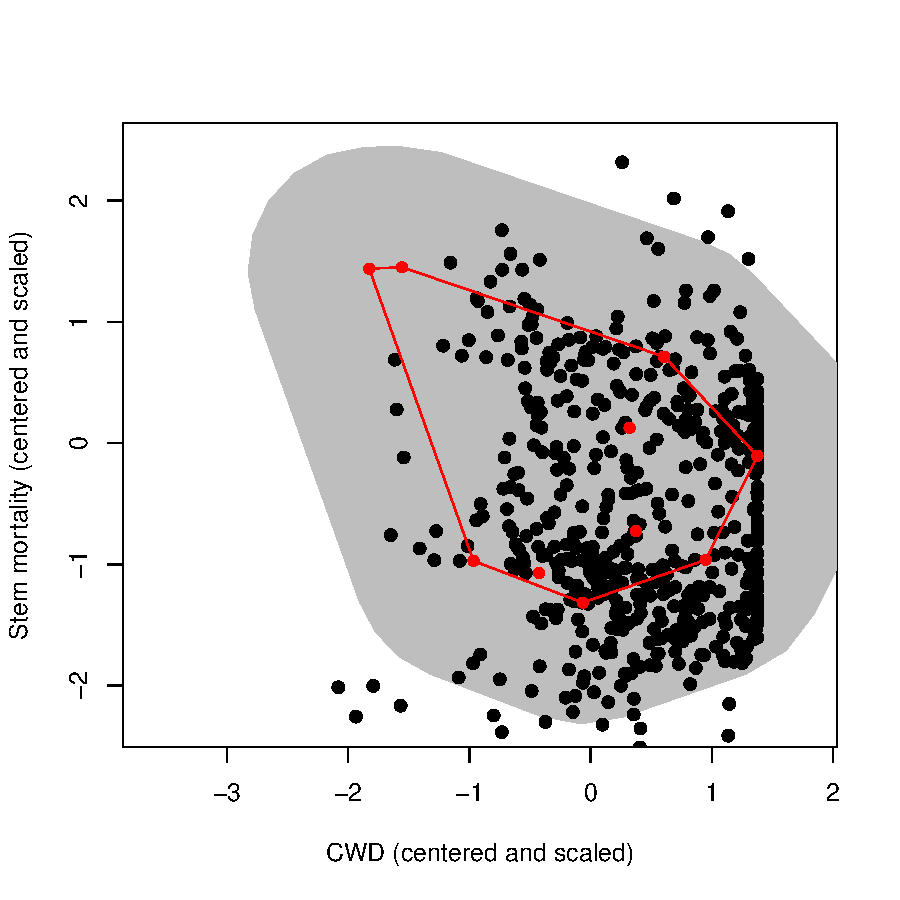
\includegraphics{rticle_tmfo_functional_files/figure-latex/pixel_choice-1.pdf}

\subsection{Goodness of predictions}\label{goodness-of-predictions}

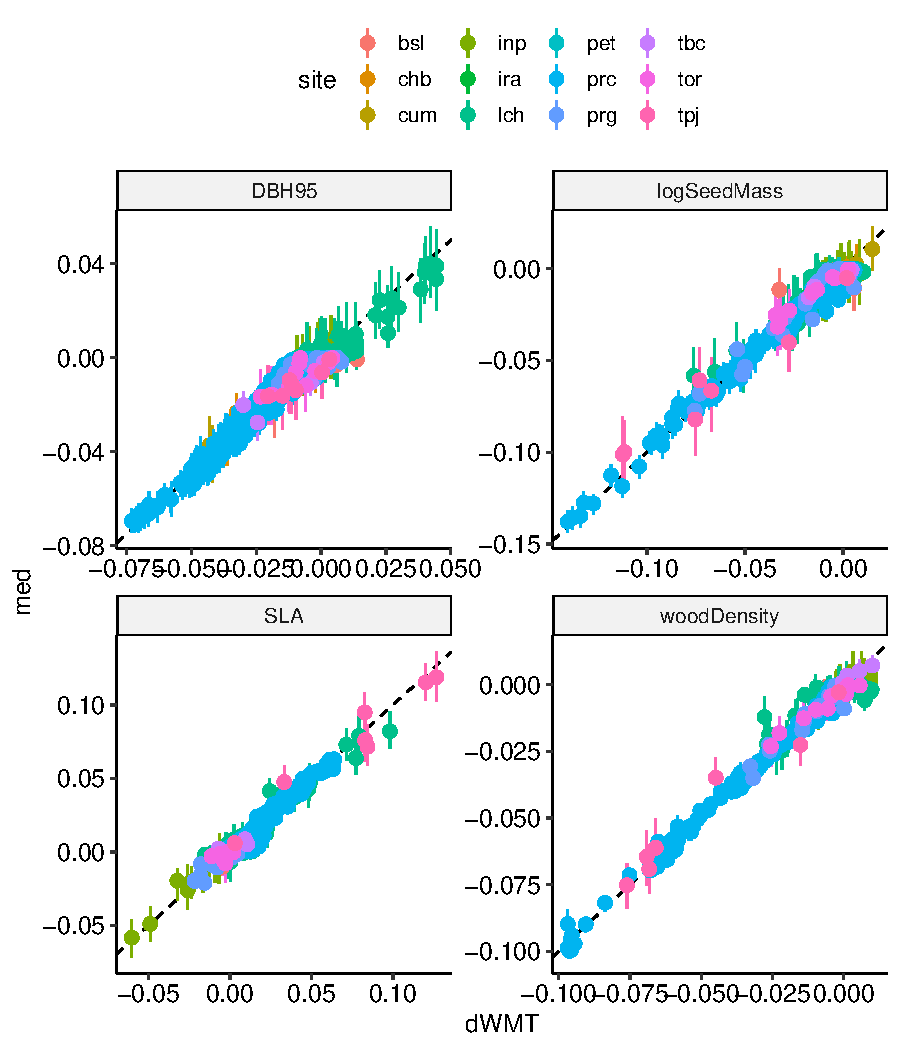
\includegraphics{rticle_tmfo_functional_files/figure-latex/gof-1.pdf}

\subsection{Predictions}\label{predictions-1}

\begin{figure}
\centering
\includegraphics{rticle_tmfo_functional_files/figure-latex/pred_obs-1.pdf}
\caption{\label{sfig:pred_traj} Observed values against trajectories of
CMT predicted with our model.}
\end{figure}

\subsection{Large trees' CMT
trajectories}\label{large-trees-cmt-trajectories}

\begin{figure}
\centering
\includegraphics{rticle_tmfo_functional_files/figure-latex/obs_large-1.pdf}
\caption{\label{sfig:pred_traj} Observed CMT trajectories of large trees
(\textgreater{} 35 cm dbh).}
\end{figure}

Here we tested the effect of removing one site on final parameter
posteriors. All sites were removed sequentially and the model was
re-calibrated with this new subset of the original data. Covariates
effects (intercept, \emph{seas}: seasonality of precipitations and
\emph{smort}: stem turnover rate) are reported for each site removal (y
axis), for each trait.

\includegraphics{rticle_tmfo_functional_files/figure-latex/loo-1.pdf}

\section*{References}\label{references}
\addcontentsline{toc}{section}{References}

\hypertarget{refs}{}
\hypertarget{ref-Aleixo2019}{}
Aleixo, Izabela, Darren Norris, Lia Hemerik, Antenor Barbosa, Eduardo
Prata, Flávia Costa, and Lourens Poorter. 2019. ``Amazonian rainforest
tree mortality driven by climate and functional traits.'' \emph{Nature
Climate Change}.
doi:\href{https://doi.org/10.1038/s41558-019-0458-0}{10.1038/s41558-019-0458-0}.

\hypertarget{ref-Antonelli2018}{}
Antonelli, Alexandre, Alexander Zizka, Fernanda Antunes Carvalho, Ruud
Scharn, Christine D. Bacon, Daniele Silvestro, and Fabien L. Condamine.
2018. ``Amazonia is the primary source of Neotropical biodiversity.''
\emph{Proceedings of the National Academy of Sciences} 115 (23):
6034--9.
doi:\href{https://doi.org/10.1073/pnas.1713819115}{10.1073/pnas.1713819115}.

\hypertarget{ref-Asner2004}{}
Asner, Gregory P, Michael Keller, and JNM Silva. 2004. ``Spatial and
temporal dynamics of forest canopy gaps following selective logging in
the eastern Amazon.'' \emph{Global Change Biology} 10 (5): 765--83.
doi:\href{https://doi.org/10.1111/j.1529-8817.2003.00756.x}{10.1111/j.1529-8817.2003.00756.x}.

\hypertarget{ref-Asner2009}{}
Asner, Gregory P., Thomas K. Rudel, T. Mitchell Aide, Ruth Defries, and
Ruth Emerson. 2009. ``A contemporary assessment of change in humid
tropical forests.'' \emph{Conservation Biology} 23 (6): 1386--95.
doi:\href{https://doi.org/10.1111/j.1523-1739.2009.01333.x}{10.1111/j.1523-1739.2009.01333.x}.

\hypertarget{ref-DeAvila2015}{}
Avila, Angela Luciana de, Ademir Roberto Ruschel, João Olegário Pereira
de Carvalho, Lucas Mazzei, José Natalino Macedo Silva, José do Carmo
Lopes, Maristela Machado Araujo, Carsten F. Dormann, and Jürgen Bauhus.
2015. ``Medium-term dynamics of tree species composition in response to
silvicultural intervention intensities in a tropical rain forest.''
\emph{Biological Conservation} 191. Elsevier B.V.: 577--86.
doi:\href{https://doi.org/10.1016/j.biocon.2015.08.004}{10.1016/j.biocon.2015.08.004}.

\hypertarget{ref-Baccini2012a}{}
Baccini, a., S. J. Goetz, W. S. Walker, N. T. Laporte, M. Sun, D.
Sulla-Menashe, J. Hackler, et al. 2012. ``Estimated carbon dioxide
emissions from tropical deforestation improved by carbon-density maps.''
\emph{Nature Climate Change} 2 (3). Nature Publishing Group: 182--85.
doi:\href{https://doi.org/10.1038/nclimate1354}{10.1038/nclimate1354}.

\hypertarget{ref-Baker2016}{}
Baker, Timothy R., Dilys M. Vela Díaz, Victor Chama Moscoso, Gilberto
Navarro, Abel Monteagudo, Ruy Pinto, Katia Cangani, et al. 2016.
``Consistent, small effects of treefall disturbances on the composition
and diversity of four Amazonian forests.'' \emph{Journal of Ecology}.
doi:\href{https://doi.org/10.1111/1365-2745.12529}{10.1111/1365-2745.12529}.

\hypertarget{ref-Baraloto2012a}{}
Baraloto, Christopher, Olivier J Hardy, C E Timothy Paine, Kyle G
Dexter, Corinne Cruaud, Luke T Dunning, Mailyn-Adriana Gonzalez, et al.
2012. ``Using functional traits and phylogenetic trees to examine the
assembly of tropical tree communities.'' \emph{Journal of Ecology} 100
(3): 690--701.
doi:\href{https://doi.org/10.1111/j.1365-2745.2012.01966.x}{10.1111/j.1365-2745.2012.01966.x}.

\hypertarget{ref-Baraloto2012}{}
Baraloto, Christopher, Bruno Hérault, C. E Timothy Paine, Hélène Massot,
Lilian Blanc, Damien Bonal, Jean-François François Molino, Eric A.
Nicolini, and Daniel Sabatier. 2012. ``Contrasting taxonomic and
functional responses of a tropical tree community to selective
logging.'' \emph{Journal of Applied Ecology} 49 (4): 861--70.
doi:\href{https://doi.org/10.1111/j.1365-2664.2012.02164.x}{10.1111/j.1365-2664.2012.02164.x}.

\hypertarget{ref-Bernhardt-Romermann2011}{}
Bernhardt-Römermann, Markus, Alan Gray, Adam J. Vanbergen, Laurent
Bergès, Andreas Bohner, Rob W. Brooker, Luc De Bruyn, et al. 2011.
``Functional traits and local environment predict vegetation responses
to disturbance: A pan-European multi-site experiment.'' \emph{Journal of
Ecology} 99 (3): 777--87.
doi:\href{https://doi.org/10.1111/j.1365-2745.2011.01794.x}{10.1111/j.1365-2745.2011.01794.x}.

\hypertarget{ref-Blaser2011}{}
Blaser, Juergen, Alastair Sarre, Duncan Poore, and Steven Johnson. 2011.
``Status of Tropical Forest Management 2011.'' Vol. 38.
\href{http://www.itto.int/news\%7B/_\%7Dreleases/id=2663}{http://www.itto.int/news\{\textbackslash{}\_\}releases/id=2663}.

\hypertarget{ref-Both2018}{}
Both, Sabine, Terhi Riutta, C. E. Timothy Paine, Dafydd M. O. Elias, R.
S. Cruz, Annuar Jain, David Johnson, et al. 2018. ``Logging and soil
nutrients independently explain plant trait expression in tropical
forests.'' \emph{New Phytologist}, September.
doi:\href{https://doi.org/10.1111/nph.15444}{10.1111/nph.15444}.

\hypertarget{ref-Brando2012}{}
Brando, Paulo M., Daniel C. Nepstad, Jennifer K. Balch, Benjamin Bolker,
Mary C. Christman, Michael Coe, and Francis E. Putz. 2012.
``Fire-induced tree mortality in a neotropical forest: The roles of bark
traits, tree size, wood density and fire behavior.'' \emph{Global Change
Biology} 18 (2): 630--41.
doi:\href{https://doi.org/10.1111/j.1365-2486.2011.02533.x}{10.1111/j.1365-2486.2011.02533.x}.

\hypertarget{ref-Cannon1994}{}
Cannon, Chuck H, David R Peart, Mark Leighton, Kuswata Kartawinata, Mark
Leighton, and R Peart David. 1994. ``The structure of lowland rainforest
after selective logging in West Kalimantan, Indonesia.'' \emph{Forest
Ecology and Management} 67 (1-3): 49--68.
doi:\href{https://doi.org/10.1016/0378-1127(94)90007-8}{10.1016/0378-1127(94)90007-8}.

\hypertarget{ref-Carpenter2015}{}
Carpenter, Bob, Andrew Gelman, Matthew D. Hoffman, Daniel Lee, Ben
Goodrich, Michael Betancourt, Marcus Brubaker, Jiqiang Guo, Peter Li,
and Allen Riddell. 2017. ``Stan : A Probabilistic Programming
Language.'' \emph{Journal of Statistical Software} 76 (1).
doi:\href{https://doi.org/10.18637/jss.v076.i01}{10.18637/jss.v076.i01}.

\hypertarget{ref-Carreno-Rocabado2012}{}
Carreño-Rocabado, Geovana, Marielos Peña-Claros, Frans Bongers, Alfredo
Alarcón, Juan Carlos Licona, and Lourens Poorter. 2012. ``Effects of
disturbance intensity on species and functional diversity in a tropical
forest.'' \emph{Journal of Ecology} 100 (6): 1453--63.
doi:\href{https://doi.org/10.1111/j.1365-2745.2012.02015.x}{10.1111/j.1365-2745.2012.02015.x}.

\hypertarget{ref-ChapinIII1997}{}
Chapin III, F. S., F S Chapin, B H Walker, R J Hobbs, D U Hooper, J H
Lawton, O E Sala, and D Tilman. 1997. ``Biotic control over the
functioning of ecosystems.'' \emph{Science} 277 (5325): 500--504.
doi:\href{https://doi.org/10.1126/science.277.5325.500}{10.1126/science.277.5325.500}.

\hypertarget{ref-Chave2009}{}
Chave, Jerome, David Coomes, Steven Jansen, Simon L Lewis, Nathan G
Swenson, and Amy E Zanne. 2009. ``Towards a worldwide wood economics
spectrum.'' \emph{Ecology Letters} 12: 351--66.
doi:\href{https://doi.org/10.1111/j.1461-0248.2009.01285.x}{10.1111/j.1461-0248.2009.01285.x}.

\hypertarget{ref-Ciemer2019}{}
Ciemer, Catrin, Niklas Boers, Marina Hirota, Jürgen Kurths, Finn
Müller-Hansen, Rafael S. Oliveira, and Ricarda Winkelmann. 2019.
``Higher resilience to climatic disturbances in tropical vegetation
exposed to more variable rainfall.'' \emph{Nature Geoscience} 12
(March). Springer US.
doi:\href{https://doi.org/10.1038/s41561-019-0312-z}{10.1038/s41561-019-0312-z}.

\hypertarget{ref-Costa-Saura2019}{}
Costa-Saura, José M., Antonio Trabucco, Donatella Spano, and Simone
Mereu. 2019. ``A height-wood-seed axis which is preserved across
climatic regions explains tree dominance in European forest
communities.'' \emph{Plant Ecology} 0123456789.
doi:\href{https://doi.org/10.1007/s11258-019-00928-x}{10.1007/s11258-019-00928-x}.

\hypertarget{ref-Crutzen2002}{}
Crutzen, Paul J. 2002. ``Geology of mankind.'' \emph{Nature} 415 (6867):
23. doi:\href{https://doi.org/10.1038/415023a}{10.1038/415023a}.

\hypertarget{ref-Davidson2012}{}
Davidson, Eric a., Alessandro C. de Araújo, Paulo Artaxo, Jennifer K.
Balch, I. Foster Brown, Mercedes M. C. Bustamante, Michael T. Coe, et
al. 2012. ``The Amazon basin in transition.'' \emph{Nature} 481 (7381):
321--28.
doi:\href{https://doi.org/10.1038/nature10717}{10.1038/nature10717}.

\hypertarget{ref-Derroire2018}{}
Derroire, Géraldine, Jennifer S. Powers, Catherine M. Hulshof, Luis E.
Cárdenas Varela, and John R. Healey. 2018. ``Contrasting patterns of
leaf trait variation among and within species during tropical dry forest
succession in Costa Rica.'' \emph{Scientific Reports} 8 (1): 1--11.
doi:\href{https://doi.org/10.1038/s41598-017-18525-1}{10.1038/s41598-017-18525-1}.

\hypertarget{ref-Espirito-Santo2014}{}
Espírito-Santo, Fernando D.B., Manuel Gloor, Michael Keller, Yadvinder
Malhi, Sassan Saatchi, Bruce Nelson, Raimundo C Oliveira Junior, et al.
2014. ``Size and frequency of natural forest disturbances and the Amazon
forest carbon balance.'' \emph{Nature Communications} 5 (March): 3434.
doi:\href{https://doi.org/10.1038/ncomms4434}{10.1038/ncomms4434}.

\hypertarget{ref-Fauset2019}{}
Fauset, Sophie, Manuel Gloor, Nikolaos M. Fyllas, Oliver L. Phillips,
Gregory P. Asner, Timothy R. Baker, Lisa Patrick Bentley, et al. 2019.
``Individual-Based Modeling of Amazon Forests Suggests That Climate
Controls Productivity While Traits Control Demography.'' \emph{Frontiers
in Earth Science} 7 (April).
doi:\href{https://doi.org/10.3389/feart.2019.00083}{10.3389/feart.2019.00083}.

\hypertarget{ref-Fick2017}{}
Fick, Stephen E, and Robert J Hijmans. 2017. ``WorldClim 2: New 1-km
spatial resolution climate surfaces for global land areas.''
\emph{International Journal of Climatology} 4315 (May): 4302--15.
doi:\href{https://doi.org/10.1002/joc.5086}{10.1002/joc.5086}.

\hypertarget{ref-Hirota2011}{}
Hirota, M., M. Holmgren, E. H. Van Nes, and M. Scheffer. 2011. ``Global
Resilience of Tropical Forest and Savanna to Critical Transitions.''
\emph{Science} 334 (6053): 232--35.
doi:\href{https://doi.org/10.1126/science.1210657}{10.1126/science.1210657}.

\hypertarget{ref-Hodgson2015}{}
Hodgson, Dave, Jenni L. McDonald, and David J. Hosken. 2015. ``What do
you mean, 'resilient'?'' \emph{Trends in Ecology and Evolution} 30 (9).
Elsevier Ltd: 503--6.
doi:\href{https://doi.org/10.1016/j.tree.2015.06.010}{10.1016/j.tree.2015.06.010}.

\hypertarget{ref-Holling1973}{}
Holling, C S. 1973. ``Resilience and Stability of Ecological Systems.''
\emph{Annual Review of Ecology and Systematics} 4 (1): 1--23.
doi:\href{https://doi.org/10.1146/annurev.es.04.110173.000245}{10.1146/annurev.es.04.110173.000245}.

\hypertarget{ref-IPCC2014}{}
IPCC. 2014. \emph{Climate Change 2014: Mitigation of Climate Change.
Contribution of Working Group III to the Fifth Assessment Report of the
Intergovernmental Panel on Climate Change}. New York, NY.

\hypertarget{ref-Jenkins2013}{}
Jenkins, C. N., S. L. Pimm, and L. N. Joppa. 2013. ``Global patterns of
terrestrial vertebrate diversity and conservation.'' \emph{Proceedings
of the National Academy of Sciences} 110 (28): E2602--E2610.
doi:\href{https://doi.org/10.1073/pnas.1302251110}{10.1073/pnas.1302251110}.

\hypertarget{ref-Johnson2018}{}
Johnson, Daniel J., Jessica Needham, Chonggang Xu, Elias C. Massoud,
Stuart J. Davies, Kristina J. Anderson-Teixeira, Sarayudh
Bunyavejchewin, et al. 2018. ``Climate sensitive size-dependent survival
in tropical trees.'' \emph{Nature Ecology and Evolution} 2 (9):
1436--42.
doi:\href{https://doi.org/10.1038/s41559-018-0626-z}{10.1038/s41559-018-0626-z}.

\hypertarget{ref-Johnson2016}{}
Johnson, Michelle O., David Galbraith, Manuel Gloor, Hannes De
Deurwaerder, Matthieu Guimberteau, Anja Rammig, Kirsten Thonicke, et al.
2016. ``Variation in stem mortality rates determines patterns of
above-ground biomass in Amazonian forests: implications for dynamic
global vegetation models.'' \emph{Global Change Biology} 22 (12):
3996--4013.
doi:\href{https://doi.org/10.1111/gcb.13315}{10.1111/gcb.13315}.

\hypertarget{ref-Johnstone2016}{}
Johnstone, Jill F., Craig D. Allen, Jerry F. Franklin, Lee E. Frelich,
Brian J. Harvey, Philip E. Higuera, Michelle C. Mack, et al. 2016.
``Changing disturbance regimes, ecological memory, and forest
resilience.'' \emph{Frontiers in Ecology and the Environment} 14 (7):
369--78. doi:\href{https://doi.org/10.1002/fee.1311}{10.1002/fee.1311}.

\hypertarget{ref-Kattge2011}{}
Kattge, J., S. Díaz, S. Lavorel, I. C. Prentice, P. Leadley, G. Bönisch,
E. Garnier, et al. 2011. ``TRY - a global database of plant traits.''
\emph{Global Change Biology} 17 (9): 2905--35.
doi:\href{https://doi.org/10.1111/j.1365-2486.2011.02451.x}{10.1111/j.1365-2486.2011.02451.x}.

\hypertarget{ref-Lavorel2002}{}
Lavorel, Sandra, and Eric Garnier. 2002. ``Predicting changes in
community composition and ecosystem functioning from plant traits:
revisiting the Holy Grail.'' \emph{Functional Ecology} 16 (5): 545--56.
doi:\href{https://doi.org/10.1046/j.1365-2435.2002.00664.x}{10.1046/j.1365-2435.2002.00664.x}.

\hypertarget{ref-Lewis2015}{}
Lewis, Simon L, David P Edwards, and David Galbraith. 2015. ``Increasing
human dominance of tropical forests.'' \emph{Science} 349 (6250):
827--32.
doi:\href{https://doi.org/10.1126/science.aaa9932}{10.1126/science.aaa9932}.

\hypertarget{ref-Lopez-Gonzalez2011}{}
Lopez-Gonzalez, Gabriela, Simon L Lewis, Mark Burkitt, and Oliver L
Phillips. 2011. ``ForestPlots.net: a web application and research tool
to manage and analyse tropical forest plot data.'' \emph{Journal of
Vegetation Science} 22 (4): 610--13.
doi:\href{https://doi.org/10.1111/j.1654-1103.2011.01312.x}{10.1111/j.1654-1103.2011.01312.x}.

\hypertarget{ref-Malhi2014}{}
Malhi, Yadvinder, Toby A. Gardner, Gregory R. Goldsmith, Miles R.
Silman, and Przemyslaw Zelazowski. 2014. ``Tropical Forests in the
Anthropocene.'' \emph{Annual Review of Environment and Resources} 39
(1): 125--59.
doi:\href{https://doi.org/10.1146/annurev-environ-030713-155141}{10.1146/annurev-environ-030713-155141}.

\hypertarget{ref-Marcon2015}{}
Marcon, Eric, and Bruno Hérault. 2015.
``\textless{}b\textgreater{}entropart\textless{}/b\textgreater{} : An
\textless{}i\textgreater{}R\textless{}/i\textgreater{} Package to
Measure and Partition Diversity.'' \emph{Journal of Statistical
Software} 67 (8).
doi:\href{https://doi.org/10.18637/jss.v067.i08}{10.18637/jss.v067.i08}.

\hypertarget{ref-Mcdowell2018}{}
Mcdowell, Nate, Craig D. Allen, Kristina Anderson-Teixeira, Paulo
Brando, Roel Brienen, Jeff Chambers, Brad Christoffersen, et al. 2018.
``Drivers and mechanisms of tree mortality in moist tropical forests.''
\emph{New Phytologist}.
doi:\href{https://doi.org/10.1111/nph.15027}{10.1111/nph.15027}.

\hypertarget{ref-Muller-Landau2010}{}
Muller-Landau, H. C. 2010. ``The tolerance-fecundity trade-off and the
maintenance of diversity in seed size.'' \emph{Proceedings of the
National Academy of Sciences} 107 (9): 4242--7.
doi:\href{https://doi.org/10.1073/pnas.0911637107}{10.1073/pnas.0911637107}.

\hypertarget{ref-Negron-Juarez2018}{}
Negrón-Juárez, R.I., JA Holm, D Magnabosco Marra, SW Rifai, WJ Riley, JQ
Chambers, CD Koven, et al. 2018. ``Vulnerability of Amazon forests to
storm-driven tree mortality.'' \emph{Environmental Research Letters} 13:
054021.
doi:\href{https://doi.org/10.1088/1748-9326/aabe9f}{10.1088/1748-9326/aabe9f}.

\hypertarget{ref-Oliver2015}{}
Oliver, Tom H., Matthew S. Heard, Nick J B Isaac, David B. Roy, Deborah
Procter, Felix Eigenbrod, Rob Freckleton, et al. 2015. ``Biodiversity
and Resilience of Ecosystem Functions.'' \emph{Trends in Ecology \&
Evolution} 30 (11). Elsevier Ltd: 673--84.
doi:\href{https://doi.org/10.1016/j.tree.2015.08.009}{10.1016/j.tree.2015.08.009}.

\hypertarget{ref-Pan2011}{}
Pan, Yude, Richard a Birdsey, Jingyun Fang, Richard Houghton, Pekka E
Kauppi, Werner a Kurz, Oliver L Phillips, et al. 2011. ``A large and
persistent carbon sink in the world's forests.'' \emph{Science (New
York, N.Y.)} 333: 988--93.
doi:\href{https://doi.org/10.1126/science.1201609}{10.1126/science.1201609}.

\hypertarget{ref-gstat}{}
Pebesma, E.J. 2004. ``Multivariable geostatistics in S: the gstat
package.'' \emph{Computers \& Geosciences} 30: 683--91.

\hypertarget{ref-Pereira2002}{}
Pereira, Rodrigo, Johan Zweede, Gregory P Asner, and Michael Keller.
2002. ``Forest canopy damage and recovery in reduced-impact and
conventional selective logging in eastern Para , Brazil.'' \emph{Forest
Ecology and Management} 168: 77--89.
doi:\href{https://doi.org/10.1016/S0378-1127(01)00732-0}{10.1016/S0378-1127(01)00732-0}.

\hypertarget{ref-Phillips2010}{}
Phillips, Oliver L., Geertje van der Heijden, Simon L. Lewis, Gabriela
López-González, Luiz E O C Aragão, Jon Lloyd, Yadvinder Malhi, et al.
2010. ``Drought-mortality relationships for tropical forests.''
\emph{New Phytologist} 187 (3): 631--46.
doi:\href{https://doi.org/10.1111/j.1469-8137.2010.03359.x}{10.1111/j.1469-8137.2010.03359.x}.

\hypertarget{ref-Piponiot2016}{}
Piponiot, Camille, Antoine Cabon, Laurent Descroix, Aurélie Dourdain,
Lucas Mazzei, Benjamin Ouliac, Ervan Rutishauser, Plinio Sist, and Bruno
Hérault. 2016. ``A methodological framework to assess the carbon balance
of tropical managed forests.'' \emph{Carbon Balance and Management} 11
(1). Springer International Publishing: 15.
doi:\href{https://doi.org/10.1186/s13021-016-0056-7}{10.1186/s13021-016-0056-7}.

\hypertarget{ref-Piponiot2019}{}
Piponiot, Camille, Edna Rödig, Francis E Putz, Ervan Rutishauser, Plinio
Sist, Nataly Ascarrunz, Lilian Blanc, et al. 2019. ``Can timber
provision from Amazonian production forests be sustainable?''
\emph{Environmental Research Letters} 14 (6). IOP Publishing: 064014.
doi:\href{https://doi.org/10.1088/1748-9326/ab195e}{10.1088/1748-9326/ab195e}.

\hypertarget{ref-Poorter2003}{}
Poorter, L, F Bongers, F J Sterck, and H Wöll. 2003. ``Architecture of
53 rain forest tree species differing in adult stature and shade
tolerance.'' \emph{Ecology} 84 (3): 602--8.
\href{http://www.esajournals.org/doi/abs/10.1890/0012-9658(2003)084\%5B0602:AORFTS\%5D2.0.CO;2}{http://www.esajournals.org/doi/abs/10.1890/0012-9658(2003)084{[}0602:AORFTS{]}2.0.CO;2}.

\hypertarget{ref-Poorter2008a}{}
Poorter, L, S J Wright, H Paz, D D Ackerly, R Condit, G
Ibarra-Manriquez, K E Harms, et al. 2008. ``Are functional traits good
precictors of demographic rates? Evidence from five neotropical
forests.'' \emph{Ecology} 89 (7): 1908--20.
doi:\href{https://doi.org/10.1890/07-0207.1}{10.1890/07-0207.1}.

\hypertarget{ref-Poorter2005a}{}
Poorter, Lourens, and Simmoné A. Rose. 2005. ``Light-dependent changes
in the relationship between seed mass and seedling traits: A
meta-analysis for rain forest tree species.'' \emph{Oecologia} 142 (3):
378--87.
doi:\href{https://doi.org/10.1007/s00442-004-1732-y}{10.1007/s00442-004-1732-y}.

\hypertarget{ref-Poorter2019}{}
Poorter, Lourens, Danaë M. A. Rozendaal, Frans Bongers, Jarcilene S. de
Almeida-Cortez, Angélica María Almeyda Zambrano, Francisco S. Álvarez,
José Luís Andrade, et al. 2019. ``Wet and dry tropical forests show
opposite successional pathways in wood density but converge over time.''
\emph{Nature Ecology \& Evolution}.
doi:\href{https://doi.org/10.1038/s41559-019-0882-6}{10.1038/s41559-019-0882-6}.

\hypertarget{ref-Quesada2012}{}
Quesada, C. a., O. L. Phillips, M. Schwarz, C. I. Czimczik, T. R. Baker,
S. Patiño, N. M. Fyllas, et al. 2012. ``Basin-wide variations in Amazon
forest structure and function are mediated by both soils and climate.''
\emph{Biogeosciences} 9 (6): 2203--46.
doi:\href{https://doi.org/10.5194/bg-9-2203-2012}{10.5194/bg-9-2203-2012}.

\hypertarget{ref-RDevelopementTeam2018}{}
R Developement Core Team. 2018. ``R: A Language and Environment for
Statistical Computing.'' \emph{R Foundation for Statistical Computing},
Lecture notes in physics,. Berlin, Heidelberg: Springer Berlin
Heidelberg.
doi:\href{https://doi.org/10.1007/978-3-540-74686-7}{10.1007/978-3-540-74686-7}.

\hypertarget{ref-Rejou-Mechain2017}{}
Réjou-Méchain, Maxime, Ariane Tanguy, Camille Piponiot, Jérôme Chave,
and Bruno Hérault. n.d. ``BIOMASS: An R Package for estimating
above-ground biomass and its uncertainty in tropical forests.''
\emph{Methods in Ecology and Evolution}.

\hypertarget{ref-Rutishauser2016}{}
Rutishauser, Ervan, Bruno Hérault, Pascal Petronelli, and Plinio Sist.
2016. ``Tree Height Reduction After Selective Logging in a Tropical
Forest.'' \emph{Biotropica} 48 (3): 285--89.
doi:\href{https://doi.org/10.1111/btp.12326}{10.1111/btp.12326}.

\hypertarget{ref-Sist2015}{}
Sist, Plinio, Ervan Rutishauser, Marielos Peña-Claros, Alexander
Shenkin, Bruno Hérault, Lilian Blanc, Christopher Baraloto, et al. 2015.
``The Tropical managed Forests Observatory: A research network
addressing the future of tropical logged forests.'' \emph{Applied
Vegetation Science} 18: 171--74.
doi:\href{https://doi.org/10.1111/avsc.12125}{10.1111/avsc.12125}.

\hypertarget{ref-Slik2015}{}
Slik, J W Ferry, Víctor Arroyo-Rodríguez, Shin-ichiro Aiba, Patricia
Alvarez-Loayza, Luciana F Alves, Peter Ashton, Patricia Balvanera, et
al. 2015. ``An estimate of the number of tropical tree species.''
\emph{Proceedings of the National Academy of Sciences} 112 (24).
doi:\href{https://doi.org/10.1073/pnas.1423147112}{10.1073/pnas.1423147112}.

\hypertarget{ref-Staal2018}{}
Staal, Arie, Obbe A. Tuinenburg, Joyce H. C. Bosmans, Milena Holmgren,
Egbert H. van Nes, Marten Scheffer, Delphine Clara Zemp, and Stefan C.
Dekker. 2018. ``Forest-rainfall cascades buffer against drought across
the Amazon.'' \emph{Nature Climate Change} 8 (June). Springer US: 1.
doi:\href{https://doi.org/10.1038/s41558-018-0177-y}{10.1038/s41558-018-0177-y}.

\hypertarget{ref-TerSteege2013}{}
Ter Steege, Hans, Nigel C a Pitman, Daniel Sabatier, Christopher
Baraloto, R. P. Salomao, Juan Ernesto Guevara, O. L. Phillips, et al.
2013. ``Hyperdominance in the Amazonian Tree Flora.'' \emph{Science} 342
(6156): 1243092--2.
doi:\href{https://doi.org/10.1126/science.1243092}{10.1126/science.1243092}.

\hypertarget{ref-Verburg2003}{}
Verburg, René, and Clara van Eijk-Bos. 2003. ``Effects of selective
logging on tree diversity, composition and plant functional type
patterns in a Bornean rain forest.'' \emph{Journal of Vegetation
Science} 14 (1): 99--110.
doi:\href{https://doi.org/10.1111/j.1654-1103.2003.tb02132.x}{10.1111/j.1654-1103.2003.tb02132.x}.

\hypertarget{ref-Violle2007}{}
Violle, Cyrille, Marie-laure Navas, Denis Vile, Elena Kazakou, Claire
Fortunel, Irène Hummel, and Eric Garnier. 2007. ``Let the concept of
trait be functional!'' \emph{Oikos} 116 (5): 882--92.
doi:\href{https://doi.org/10.1111/j.2007.0030-1299.15559.x}{10.1111/j.2007.0030-1299.15559.x}.

\hypertarget{ref-Wright2004}{}
Wright, Ian J., Peter B. Reich, Mark Westoby, David D. Ackerly, Zdravko
Baruch, Frans Bongers, Jeannine Cavender-Bares, et al. 2004. ``The
worldwide leaf economics spectrum.'' \emph{Nature} 428 (6985): 821--27.
doi:\href{https://doi.org/10.1038/nature02403}{10.1038/nature02403}.

\hypertarget{ref-Wright2005}{}
Wright, S. Joseph. 2005. ``Tropical forests in a changing environment.''
\emph{Trends in Ecology and Evolution} 20 (10): 553--60.
doi:\href{https://doi.org/10.1016/j.tree.2005.07.009}{10.1016/j.tree.2005.07.009}.

\hypertarget{ref-Zanne2009}{}
Zanne, A. E., G. Lopez-Gonzalez, D.A. A Coomes, J. Ilic, S. Jansen,
Simon L S.L. Lewis, R.B. B Miller, N.G. G Swenson, M.C. C Wiemann, and
Jerome Chave. 2009. ``Global wood density database.'' Vol. 235.
doi:\href{https://doi.org/10.5061/dryad.234}{10.5061/dryad.234}.

\end{document}


